%
% Poster latex file for ADASS 2018
% Pey Lian Lim (lim@stsci.edu)
% Eric Jeschke (eric@naoj.org)
%
% [top-level file]
\nonstopmode

\documentclass[]{article}
\usepackage{graphicx}
% where can I find the graphics that will be imported for this version
\graphicspath{{./figures/}}

% Using \fbox you can draw a nice razor-thin border around images
\setlength\fboxsep{0pt}
\setlength\fboxrule{0.5pt}

% in case you want to embed any hyperlinks
%\usepackage{hyperref}

% for + and - signs in setting width etc
\usepackage{calc}

% scalable fonts
\usepackage[quiet]{fontspec}
\setmainfont[Mapping=tex-text,Scale=2.1]{DejaVu Serif}
\setsansfont[Mapping=tex-text,Scale=2.1]{DejaVu Sans}
\setmonofont[Mapping=tex-text,Scale=2.1]{DejaVu Sans Mono}
%\setmainfont[Mapping=tex-text,Scale=1.0]{Times New Roman}
%setsansfont[Mapping=tex-text,Scale=1.0]{Arial}
%setmonofont[Mapping=tex-text,Scale=1.0]{Courier New}

% for multiple columns
\usepackage{multicol}

% fancy boxes
\usepackage{fancybox}

% uncomment the actual desired size
%\def\mypaperwidth{33.11in} \def\mypaperheight{46.81in}    % A0
\def\mypaperwidth{27.83in} \def\mypaperheight{39.37in}     % B1
%\def\mypaperwidth{23.39in} \def\mypaperheight{33.1124in}  % A1
%\def\mypaperwidth{8.27in} \def\mypaperheight{11.69in}  % A4
\def\imgwd{6.0in}  % define image widths
% margin around edge of page
\def\mymargin{1in}

%% \def\mypaperwidth{11in} \def\mypaperheight{17.0in}     % Tabloid
%% \def\imgwd{2.5in}  % define image widths
%% \def\mymargin{0.25in}

% painful TeX calculation of 2*margin
\dimen87=\mymargin
\multiply\dimen87 by 2
\def\mydblmargin{\dimen87}

\usepackage[paperwidth=\mypaperwidth, paperheight=\mypaperheight,
            % margins are calculated from the trim + no print area
            top=\mymargin, bottom=\mymargin,
            left=\mymargin, right=\mymargin]{geometry}

\begin{document}

% dimensions of main writing area of page
\setlength{\textwidth}{\mypaperwidth-\mydblmargin}
%\setlength{\textwidth}{13in}
\setlength{\textheight}{\mypaperheight-\mydblmargin}

% TeX defines the content to begin at 1in offset from the side and
% top of the document (seemingly somewhat independent of margin
% settings).  These specify offsets to be added to the 1in defaults.
% You can calculate these or just tweak them until you get the result
% that you like.
\setlength{\hoffset}{-1.0in}
\setlength{\voffset}{-1.0in}

% width of margin notes area
\setlength{\marginparwidth}{0in}
% distance between margin and paragraph
\setlength{\marginparsep}{0in}

% footer configuration
\setlength{\footskip}{1em}

% header configuration
\setlength\headheight{0in}
\setlength\headsep{1em}

% margin tweaking
\setlength{\topmargin}{0.0in}
\setlength{\oddsidemargin}{1in}
% LEFT margin on even pages
\setlength{\evensidemargin}{1in}

% define explicitly set paragraph spacing
\newcommand{\para}{\vspace*{1em}}

\title{{\tt stginga}: Ginga Plugins for Data Analysis and Quality Assurance of
            HST and JWST Science Data}
\author{P. L. Lim (STScI) and E. Jeschke (NAOJ)}

% paragraph indentations
\setlength{\parindent}{0in}
% amount of space before each new paragraph begins
\setlength{\parskip}{0pt}

% comment to force even justification
\raggedright

%\begin{document}

\pagestyle{empty}

% interior facing page for book version
\begin{minipage}[t]{0.8\linewidth}
  \vspace{0pt}
\begin{center}
{\huge {\tt stginga}: Ginga Plugins for Data Analysis and Quality Assurance of
            HST and JWST Science Data }\\

\vspace*{1.5em}
Pey Lian Lim ({\tt lim@stsci.edu}),
Space Telescope Science Institute \\
Eric Jeschke ({\tt eric@naoj.org}),
National Astronomical Observatory of Japan
\end{center}
\end{minipage}
\hfill
\begin{minipage}[t]{0.15\linewidth}
  \vspace{0pt}
  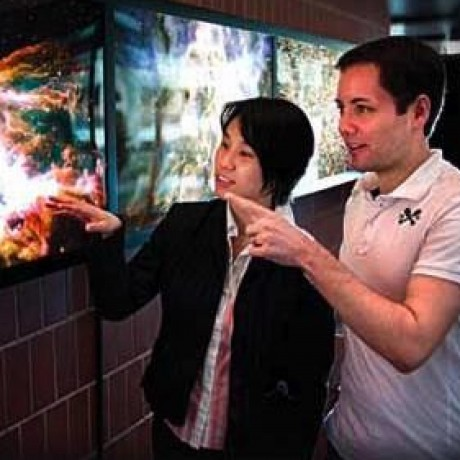
\includegraphics[width=2in]{pllim} \\
  {P. L. Lim}
\end{minipage}
%\vspace*{0in}
\vspace*{2em}

\noindent\hrulefill

\raggedcolumns
\setlength{\columnseprule}{1pt}
\setlength{\columnsep}{2em}

\medskip
\begin{multicols}{3}

\section*{Abstract}
{\tt stginga}\cite{stginga} is an image visualization package to assist
in data analysis and quality assurance of science data from Hubble Space
Telescope (HST) and James Webb Space Telescope (JWST).  It is based on the
Ginga\cite{ginga} toolkit for building scientific viewers.
In this poster, we will describe the main plugins developed for data
analysis and quality assurance tasks with {\tt stginga}.  We also discuss the
basic outline of writing a Ginga plugin, with pointers to documentation
and examples.

\section*{Introduction}

\begin{center}
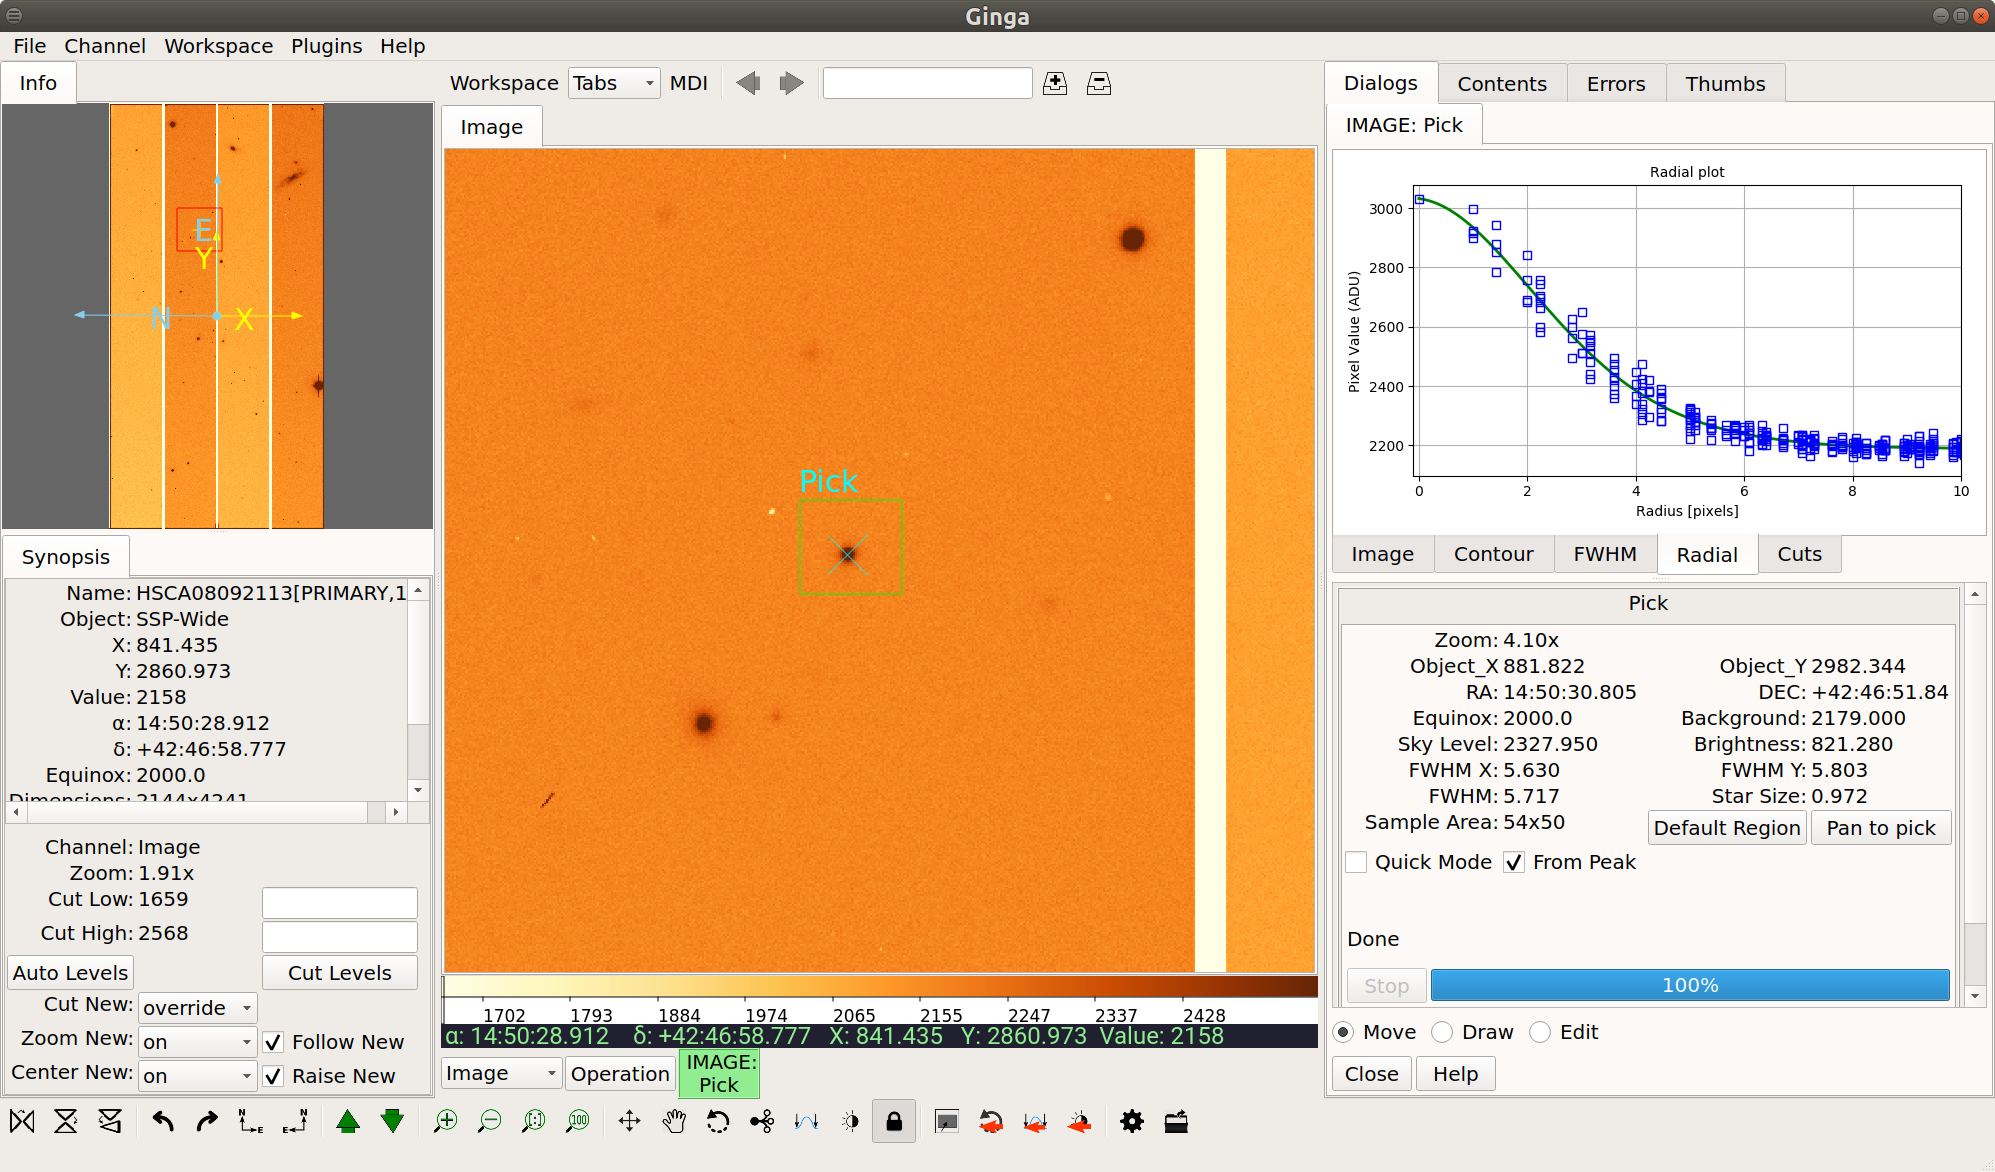
\includegraphics[width=8in]{ref_viewer}
\label{fig:refviewer}
\vspace*{0.4em}
{\small\em Figure 1: The Ginga reference viewer.}
\end{center}

\para
Ginga\cite{Jeschke15A} is a Python package that
implements a toolkit for building scientific viewers.  It provides
a \emph{reference viewer} (see Fig. 1), which features
a plugin architecture in which nearly every graphical feature of the
program is implemented by a Python plugin.
By implementing some new plugins for the HST and JWST data analysis and
quality assurance tasks, and combining these with a curated selection of
the distributed ``stock'' plugins, we were able to fairly quickly
develop a tool for use in the HST and JWST community.

\para
The reference viewer separates image data into virtual holding pens
called \emph{channels}, named and organized by the user.
Plugins are categorized as \emph{global} or \emph{local}.  A global
plugin applies to all images across all channels: only one instance can
be opened in the whole Ginga session, whereas a local plugin is
associated with the channel it is started from: one instance can be
opened per channel and different instances can be configured separately
in the same Ginga session.
%% Plugins are currently not available when Ginga is used as part of Jupyter
%% Notebook/Lab. However, they are usable in a limited way via Ginga's remote
%% control (RC) interface, which will not be covered here.

\para
Currently, all the plugins in {\tt stginga} are local plugins.
As with many Ginga plugins, they can be customized via a file in the
user's home directory:
{\tt \textasciitilde/.ginga/plugin\_{\em PluginName}.cfg}.
Some plugins currently in Ginga originated from {\tt stginga}
(e.g., {\em ChangeHistory}, {\em SaveImage}, {\em TVMark}, and {\em TVMask})
when they were identified to be useful in general beyond HST or JWST.
The viewer can use different toolkit \emph{backends};
all the screenshots shown in this poster used Qt5 backend, although they should
also work with the Qt4, PySide, GTK 2, and GTK 3 backends.

\section*{BackgroundSub}

\begin{center}
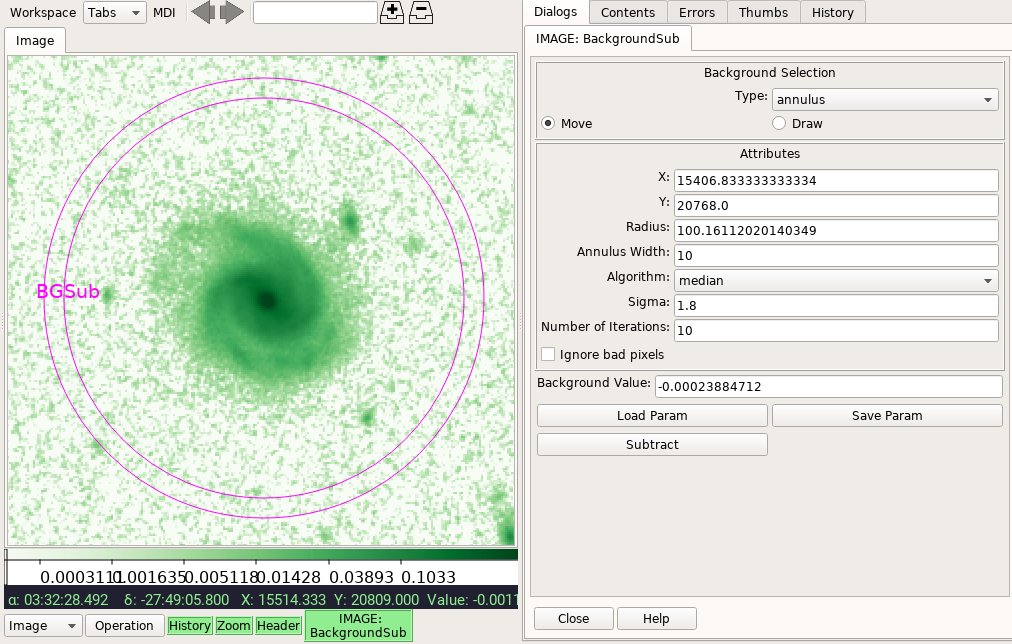
\includegraphics[width=8in]{plugin_backgroundsub} \\
\vspace*{0.4em}
\label{fig:plugin_backgroundsub}
{\small\em Figure 2: BackgroundSub plugin for background subtraction.}
\end{center}

\para
{\em BackgroundSub} (see Fig. 2) is used to calculate and subtract background
value. User draws a shape (e.g., annulus) to define
the region from which background is calculated. In the ``Attributes'' box,
parameters controlling the calculation can be adjusted.
As user modifies the region or changes the parameters, background value would
be recalculated accordingly.
Optionally, if a data quality (DQ) extension is available, pixels marked as
``not good'' can be excluded from calculations as well.
Subtraction parameters can be saved to a JSON file, which then can be reloaded.

\para
Finally, if desired, the calculated background can be subtracted off
the displayed image in Ginga.
However, the subtracted image only exists in an in-memory cache in Ginga;
if the cache fills up Ginga will eventually eject the image if it is not
being viewed.
To save the subtracted image out to a different file, use the {\em SaveImage}
plugin in Ginga.
As of this writing, {\em BackgroundSub} only handles constant
background, therefore unsuitable for when background has a gradient or a
pattern.

\section*{BadPixCorr}

\begin{center}
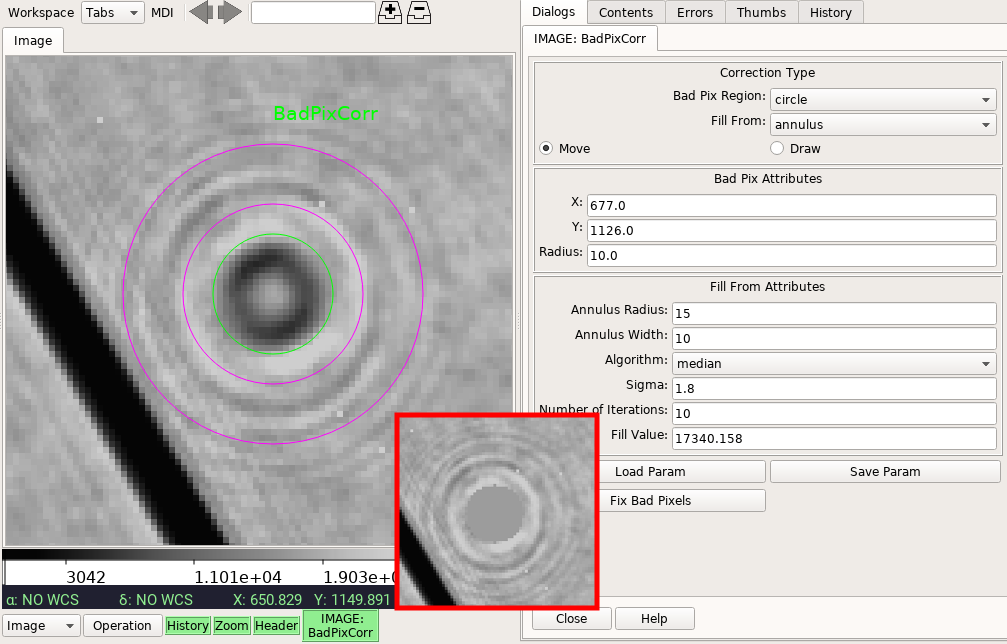
\includegraphics[width=8in]{plugin_badpixcorr.png}
\label{fig:plugin_badpixcorr}
\vspace*{0.4em}
{\small\em Figure 3: BadPixCorr plugin for bad pixel correction.}
\end{center}

\para
{\em BadPixCorr} (see Fig. 3) is a plugin for performing interactive bad pixel
correction on an image. Currently, it only handles fixing a single bad pixel or
bad pixels within a circular region.
The bad pixel(s) can be filled either by a user-defined constant, a constant
calculated from an annulus (not unlike {\em BackgroundSub}), or Scipy
{\tt griddata} interpolation using the annulus.
If DQ extension is present, the corresponding DQ flags will also be set
to the given new flag value (default is 0 for ``good'').

\para
Like {\em BackgroundSub}, it supports saving/loading parameters to/from
JSON file and the corrected image only exists in the Ginga in-memory cache;
if the cache fills up Ginga will eventually eject the image if it is not
in use.  To save the result image, use {\em SaveImage}.

\section*{DQInspect}

\begin{center}
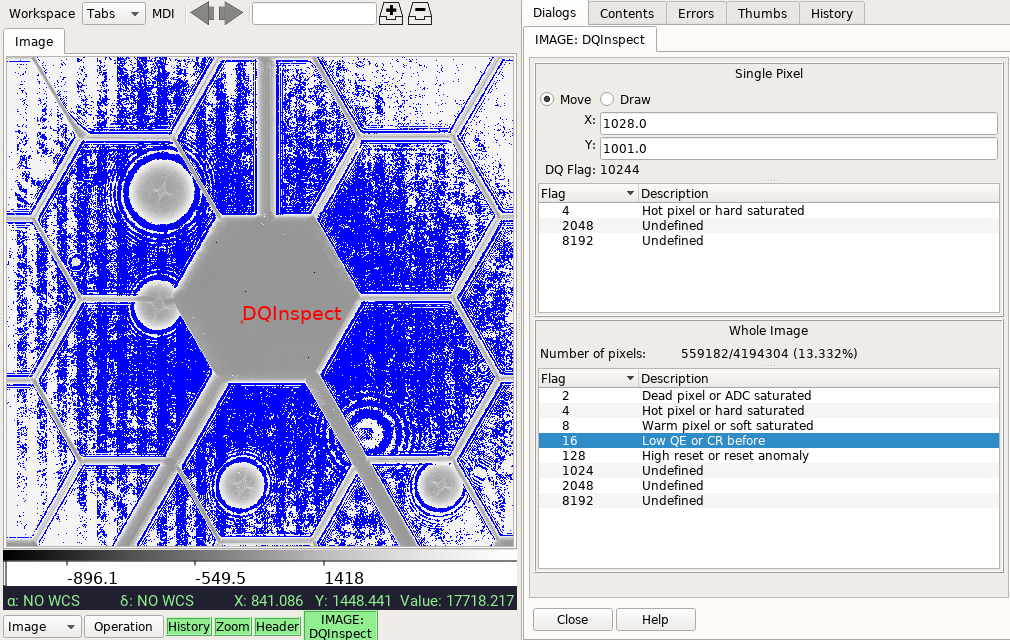
\includegraphics[width=8in]{plugin_dqinspect} \\
\vspace*{0.4em}
\label{fig:plugin_dqinspect}
{\small\em Figure 4: DQInspect plugin for data quality inspection.}
\end{center}

\para
{\em DQInspect} (see Fig. 4) is used to visualize the associated DQ
array stored as an HDU within an image.
It shows the different DQ flags (top table) that went into a selected pixel
(marked by a red ``x'')
and also the overall mask of the selected DQ flag(s)
(blue pixels; bottom table).
For overall mask, when multiple flags are selected, each flag is assigned a
different mask color at a reduced opacity for each.
User has the option to customize flag definitions for different instruments.

\section*{SNRCalc}

{\em SNRCalc} (see Fig. 5) is used to calculate Signal-to-Noise Ratio
(SNR) and Surface Background Ratio (SBR) on an image.
Given the selected science ({\em S}) and background ({\em B}) regions,
SBR is defined by Ball Aerospace\cite{sbr} as the median of {\em S}
divided by the standard deviation of {\em B}.
If the image has an accompanying error ({\em E}) extension, SNR can also
be calculated by dividing {\em S} by {\em E} over the same region and
then computing its min, max, and mean.

\para
\begin{center}
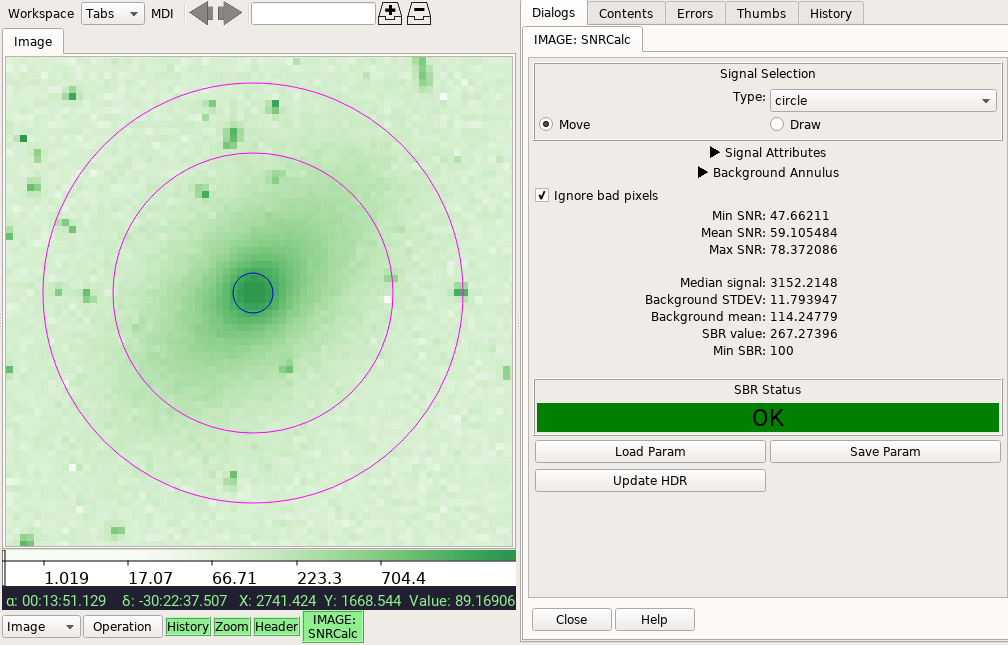
\includegraphics[width=8in]{plugin_snrcalc} \\
\vspace*{0.4em}
\label{fig:plugin_snrcalc}
{\small\em Figure 5: SNRCalc plugin for SNR calculation.}
\end{center}

\para
While SNR is more popular, SBR is useful for an image without existing or
reliable error values. User may define a minimum limit for SBR check,
so that the GUI can provide a quick visual indication on whether the
selected region achieves the desired SBR or not.
As part of the statistics, mean background value is also
provided, albeit not used in SBR nor SNR calculations.
Optionally, if DQ extension is available, pixels marked as
``not good'' can be excluded from calculations as well.

\para
Like {\em BackgroundSub}, it supports saving/loading parameters to/from
JSON file.
Calculated values can be saved in the image header using the ``Update HDR''
button.
The image with updated header only exists in the Ginga cache until it
is forced out by viewing other images; to save it, use {\em SaveImage}.

\section*{Writing a Ginga plugin}

% TODO: Polish text and update link.
% NOTE: Link is broken into 2 lines to prevent overfull \hbox
\para
Instructions for writing a plugin is available at
{\tt https://bit.ly/writeplugins}.
Existing plugins in Ginga and {\tt stginga} code repositories can be used as
examples. It is recommended that you play with the existing ones and
choose one that is the closest to your desired functionality as a
starting point.

\subsection*{Local plugins}
A local plugin at its simplest is a Python class defined in a file.
The class should inherit from {\tt ginga.GingaPlugin.LocalPlugin}
and provide {\tt \_\_init\_\_()}, {\tt build\_gui()}, {\tt start()},
and {\tt stop()} methods.  These methods are used to initialize the
plugin, build the user interface, and to do any necessary tasks at the
start and stop of the plugin, respectively. Typically, you would also
want to implement the {\tt redo()} method, which is called when there are
new data loaded into the viewer to which the running plugin should respond.

\para
Inside the file, any modules that are available in the user's Python
environment may be imported and used, allowing huge flexibility in
the kinds of things a plugin can do; i.e., open files, connect to
sockets or other communication frameworks, or call a myriad of
astronomical Python packages.  It also has a reference to the viewer with
which it is associated so it can access the viewer data (as Numpy array)
and can manipulate canvas overlays with graphics on the viewer (as shown
in the sections above) or manipulate the viewer settings (e.g., panning,
scale, color map).

\subsection*{Global plugins}
Writing a global plugin is similiar to the process for writing a local
one. The difference is that the plugin ostensibly must be able to
update its state when the user switches channels, since there is only
one instance of the plugin allowed to be open; There are callbacks
for which you can register to be alerted of these events. Otherwise,
the API is quite similar to that of a local plugin.

\subsection*{Distributing plugins}
When you want to distribute your plugin(s), the best way is to use
the {\tt ginga-plugin-template} \cite{plugin-template}.
This template allows one
or more plugins to be installed as a separate package, and be
discovered by the reference viewer when it starts up.  If you want
more control over the layout of the viewer and the set of included
plugins, you can follow the path blazed by {\tt stginga} and make your own
startup script for the reference viewer with a curated mix of the
stock plugins with your own.

\section*{Conclusion}

{\tt stginga} utilizes Ginga plugins to support HST and JWST data analysis,
which includes background subtraction, bad pixel correction, DQ flags
inspection, and signal-to-noise calculations.

\para
Writing Ginga plugins can be an expedient way to develop graphical data
analysis and quality assurance tasks, by leveraging the combination of
Python, a lean Ginga plugin API, and the burgeoning number of open-source
astronomical Python modules.

\para
Both {\tt stginga} and {\tt ginga} are installable via {\tt pip}. Alternately,
if you use {\tt conda}, they are also available on AstroConda\cite{astroconda},
in addition to {\tt ginga} being in  {\tt conda-forge} too. Their development
versions could be cloned from GitHub. Both are open-source and licensed under
3-clause BSD.

\bibliographystyle{abbrv}
\bibliography{poster}

\end{multicols}

\end{document}
